\documentclass[12pt,reqno]{amsart}
% \usepackage[pdfborder={0 0 0.5 [3 2]}]{hyperref}%
\usepackage[left=1in,right=1in,top=1in,bottom=1.5in]{geometry}%
\usepackage{amssymb}
\usepackage{amsthm}
\usepackage{graphicx}
\usepackage{enumerate}
\usepackage{float}
\usepackage{subfiles}
\usepackage{thmtools, thm-restate}
\usepackage{bm}
\usepackage[stable]{footmisc}

\usepackage{packages}

\newtheorem{theorem}{Theorem}
\newtheorem{lemma}[theorem]{Lemma}
\newtheorem{corollary}{Corollary}

\theoremstyle{definition}
\newtheorem{definition}[theorem]{Definition}
\newtheorem{example}[theorem]{Example}
\newtheorem{hypothesis}{Hypothesis}


\theoremstyle{remark}
\newtheorem{remark}[theorem]{Remark}

\def\noi{\noindent}
\def\T{{\mathbb T}}
\def\R{{\mathbb R}}
\def\N{{\mathbb N}}
\def\Z{{\mathbb Z}}
\def\C{{\mathbb C}}
\def\Q{\mathbb{Q}}

\DeclareMathOperator{\spn}{span}
\DeclareMathOperator{\ran}{ran}
\DeclareMathOperator{\dm}{dim}

\newcommand{\vK}{\bm{\mathit{K}}}
\newcommand{\calP}{\mathcal{P}}
\newcommand{\calA}{\mathcal{A}}


\begin{document}

\section{Research Summary}

Solitons are localized disturbances in a medium which maintain their shape as they propagate at a constant velocity. Although they were originally discovered as a water wave phenomenon, they have applications in many fields such as fiber optics, plasma physics, and quantum mechanics; they can also be used for models in biology and neuroscience. More generally, many weakly nonlinear, dispersive PDEs admit soliton solutions.

I am interested in multi-solitons, which are disturbances which resemble multiple, well-separated copies of a single soliton. Since these structures also maintain their shape as time evolves, it appears at first glance that the individual solitons do not interact. The underlying dynamics, however, is inherently nonlinear. This is revealed when we perturb a multi-soliton. If we ``bump'' one of the solitons, many different behaviors are possible. For example, the two solitons could fly apart, the solitons could oscillate about their midpoint, or the system could decay to back to the original configuration. I am interested in the stability of multi-soliton structures.

The first step to understanding stability of multi-solitons is studying the spectrum resulting from linearizing the underlying PDE about one of these solutions. In all of the systems I study, the underlying single soliton state is stable. Typically, as we add another soliton to the structure, one or more additional eigenvalues are added to the spectrum. These eigenvalues are close to 0, and I refer to them as interaction eigenvalues, since they result from nonlinear interactions between neighboring solitons. For a large class of systems, this problem is solved in \cite{Sandstede1998}, where the problem of finding the interaction eigenvalues for a $n$-soliton is reduced to the finding the eigenvalues of an $n \times n$ matrix.

The systems I study are Hamiltonian. This case is not covered the results of \cite{Sandstede1998}. Additional structure is provided by the presence of a quantity which is conserved in time. This structure is very helpful, since eigenvalues must come in quartets of the form $\pm \alpha \pm \beta i$; in particular, this means that each additional set of interaction eigenvalues must come in one of the three patterns in \cref{fig:inteigpattern}
\begin{figure}[ht]
\centering
\includegraphics[width=7cm]{inteigpattern.eps}
\caption{Possible eigenvalue patterns for interaction eigenvalues.} 
\label{fig:inteigpattern}
\end{figure}
On the other hand, the presence of any eigenvalue with nonzero real part implies that there is an unstable eigenvalue. This means that Hamiltonian systems cannot be dissipative, which complicates the stability analysis. For Hamiltonian systems, optimum stability is achieved when the entire spectrum lies on the imaginary axis; in this situation, the best we can hope for is a neutral stability result. 

In my work, I look at three main examples: the fifth order Korteweg–de Vries equation (KdV5), the Chen-McKenna suspension bridge equation, and the discrete nonlinear Schrodinger equation (dNLS). The first two are PDEs on the real line, and the last is a lattice differential equation. In all three examples, I start with numerical analysis. First, I construct the multi-soliton solutions; in most cases, this involves constructing a single soliton solution, gluing copies of this together at the appropriate distances, and using a Newton solver to obtain the solution. I then use an eigenvalue solver to find the interaction eigenvalues; this involves spatial discretization, usually with Fourier or polynomial spectral methods. In the case of KdV5, I also perform numerical timestepping starting with perturbations of multi-solitons.

For my analysis, I use several mathematical tools. My primary approach is spatial dynamics. From this viewpoint, a soliton becomes a homoclinic orbit evolving in the spatial variable. Multi-solitons are multi-loop homoclinic orbits, and I construct them using Lin's method \cite{Lin2008}, a version of the Lyapunov-Schmidt method used to construct solutions which remain near a homoclinic orbit. I also construct periodic orbits and multi-loop periodic orbits this way. To find the interaction eigenvalues associated with these solutions, I use several tools, which include Lin's method \cite{Sandstede1998} and a the Krein matrix \cite{Kapitula2013a}.
  
A common theme among my work is that the interaction eigenvalue pattern is determined by the geometry of the underlying multi-soliton solution. For continuous systems, multi-solitons exist in discrete families, where the distances between consecutive peaks is, to leading order, an integer multiple of a phase parameter; this constraint is a consequence of the geometry of the unstable and stable manifolds. The interaction eigenvalue pattern is determined by these integers. For dNLS, we have no such restriction; multi-solitons exist as long as the individual solitons are well separated. Multi-solitons in dNLS, however, can be composed of ``up'' and ``down'' solitons. The eigenvalue pattern is determined by the configuration of ``ups'' and ``downs''.

\section{Fifth order KdV equation\footnote{Work with Bj\"{o}rn Sandstede}}

The 5th order KdV equation (KdV5), written in a co-moving coordinate frame with speed $c$, is a weakly nonlinear long wave approximation to capillary-gravity wave problem
\begin{equation}\label{KdV5}
u_t - \partial_x^5 u + \partial_x^3 u - c \partial_x u + 2 u \partial_x u = 0
\end{equation}
For wavespeeds $c > 0$, a symmetric soliton solution $u_1(x)$ exists \cite{pelinovsky_2011} which is orbitally stable. For $c > 1/4$, multi-soliton solutions exist \cite{Buffoni1996,SandstedeStrut}. The distance between pulses, however, is constrained by the fact that a particular alignment of the stable and unstable manifolds is required for a multi-loop homoclinic orbit to exist; this implies that the distances between consecutive peaks must (approximately) be an integer multiple of a phase parameter $\phi$ which depends on the eigenvalues of the rest state. Specifically, for each $m \geq 2$, a countable family of $m-$solitons solutions exists \cite[Theorem~3.6]{SandstedeStrut}; each of these $m-$solitons can be described by a set of $m-1$ nonnegative integers $\{ k_1, \dots, k_{m-1} \}$. The distances between consecutive peaks are $L_j \approx k_j \phi + C$, where $C$ is a constant.

I am interested in the spectral stability of these multi-solitons. The essential spectrum for all soliton solutions is the entire imaginary axis, so spectral stability of multi-solitons depends on the interaction eigenvalues. I start with numerical analysis. An exact soliton solution is known for $c = 36/169 < 1/4$ \cite{Pelinovsky2007}. I use AUTO for parameter continuation to increase $c$ until $c > 1/4$. I then splice together multiple copies of the primary pulse at the appropriate distances, and solve for the multi-pulse using Matlab. I then find the spectrum of the linearization about theses solutions using Matlab's eigenvalue solver.

The first two double pulses ($k_1 = 0$ and $k_1 = 1)$, together with their eigenvalue patterns, are shown in \cref{fig:KdV5dp}.
\begin{figure}[ht]
\centering
\begin{tabular}{ccc}
\includegraphics[width=5cm]{double12.eps}
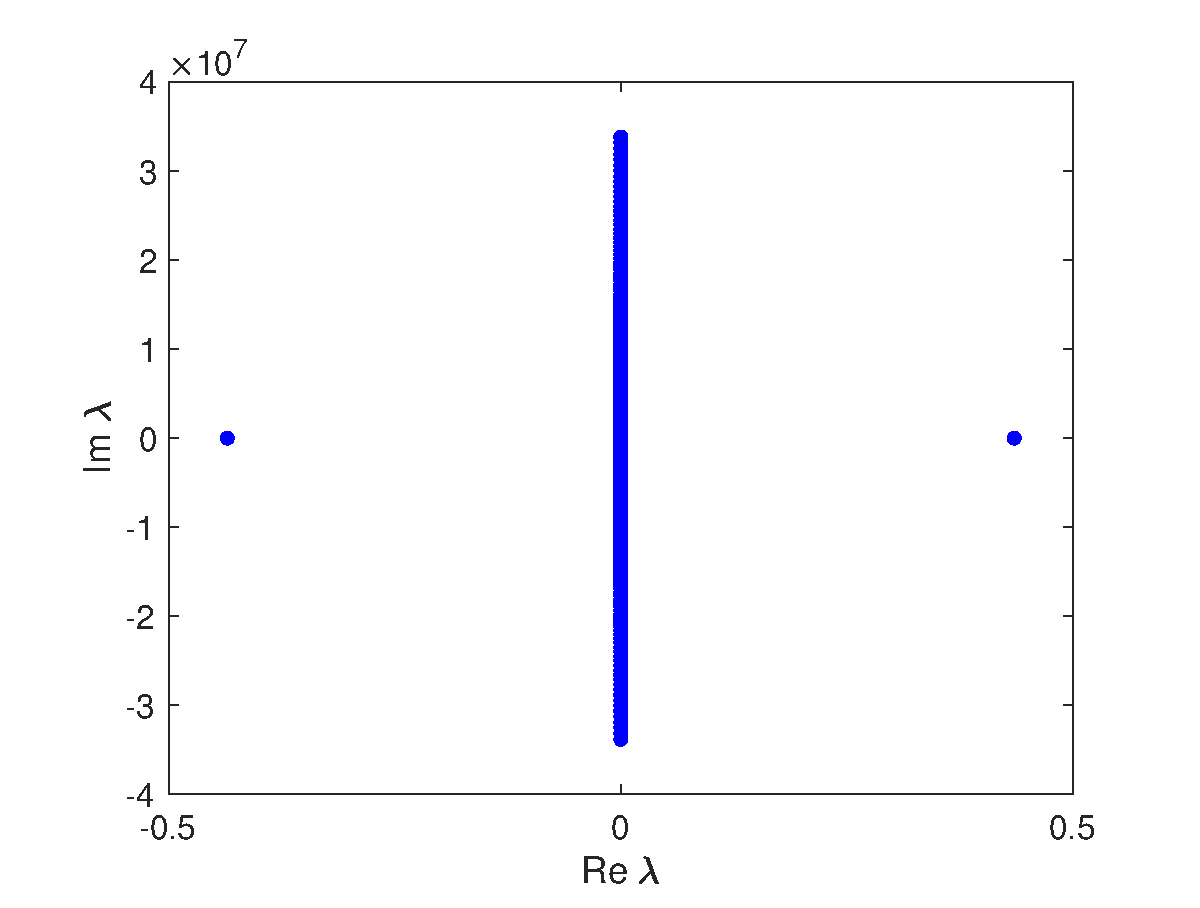
\includegraphics[width=5cm]{dpeig1.eps}
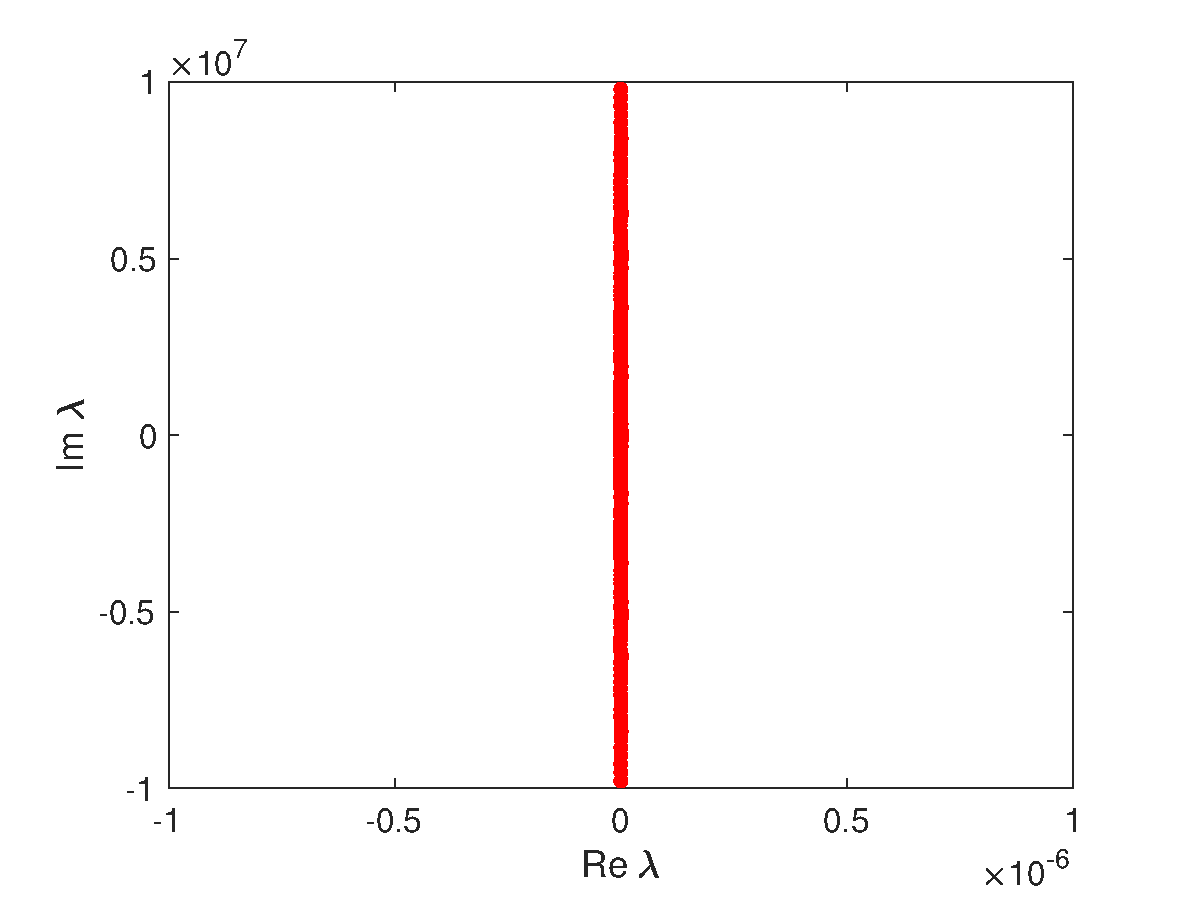
\includegraphics[width=5cm]{dpeig2.eps}
\end{tabular}
\caption{Left panel shows first two double pulse solutions to KdV5: $k_1 = 0$ (blue) and $k_1 = 1$ (red). Spectrum for $k_1 = 0$ (center panel) and $k_1 = 1$ (right panel).
 } 
\label{fig:KdV5dp}
\end{figure}
For $k_1 = 0$, there is is a pair of real interaction eigenvalues; we also see the purely imaginary essential spectrum. For $k_1 = 1$, it is difficult to locate the interaction eigenvalues, since it appears they are buried in the essential spectrum. If we zoom in around the origin, we can locate a pair of interaction eigenvalues which are purely imaginary to leading order. This pattern of alternating pairs of real and imaginary eigenvalues continues as $k_1$ increases. 

To see the implications of these eigenvalues for the PDE, we 
perform time-stepping starting with initial conditions which are close to these 2-soliton solutions. At each time point, I  compute the peak distance and its derivative, which I call the pulse relative velocity. Trajectories of this two-dimensional system are plotted in the left panel of \cref{fig:KdV5timestep}
\begin{figure}[ht]
\begin{center}
\begin{tabular}{cc}
\includegraphics[width=8cm]{phaseportrait} &
\includegraphics[width=8cm]{simplephaseportrait} \\
\end{tabular}
\caption{Phase portrait for peak relative velocity vs. peak distance for timestepping of \cref{KdV5} with initial conditions near the first four double pulses (left panel). Phase portrait of \cref{harmonicvary} (right panel)
}
\label{fig:KdV5timestep}
\end{center}
\end{figure}
This phase portrait consists of alternating saddles and centers and resembles the following planar system, which is harmonic oscillator with spatially varying restoring force.
\begin{equation}\label{harmonicvary}
\begin{aligned}
\dot{x} &= y \\
\dot{y} &= C e^{-\alpha_0 x} \sin \beta_0 x
\end{aligned}
\end{equation}
The phase portrait for this system is plotted in the right panel of \cref{fig:KdV5timestep} and is qualitatively similar to the one for the 2-solitons.

To obtain an analytical result, we adapt the procedure in \cite{Sandstede1998} and use Lin's method to construct eigenfunctions. This, requires the use of an exponentially weighted space, which breaks the Hamiltonian symmetry of the system. Thus we are only able to obtain the following limited result.

\begin{theorem}\label{KdV5unstable}
Let $u_n(x)$ be a $n$-soliton solution to KdV5 constructed with integers $\{ k_1, \dots, k_{m-1} \}$. If any of the $k_j$ is even, then there is an interaction eigenvalue with positive real part, thus $u_n(x)$ is spectrally unstable. If all the $k_j$ are odd, then there are $n-1$ pairs of interaction which are purely imaginary to leading order.
\end{theorem} 

One challenge in locating any purely imaginary interaction eigenvalues is that they would be buried in the essential spectrum. To circumvent that, I look at periodic multi-soliton solutions. From a spatial dynamics perspective, these are multi-loop periodic orbits which are close to the primary homoclinic orbit. The advantage in this case is that the essential spectrum becomes a discrete set of purely imaginary eigenvalues whose location depends only on the size of the periodic domain. One complication with this approach is that there is a possible interaction between eigenmodes corresponding to purely imaginary interaction eigenvalues and the essential spectrum if their corresponding eigenvalues become close. 

For simplicity, I will discuss periodic 2-solitons here, although we can construct periodic $m$-solitons for any $m$. We use Lin's method to construct a periodic 2-soliton by gluing together two individual solitons; this time, however, we must glue them together at both ends. First, we prove that asymmetric periodic 2-solitons bifurcate from symmetric perioid 2-solitons a series of pitchfork bifurcations. This is shown in \cref{fig:perpitchfork}.

\begin{figure}[ht]
\begin{center}
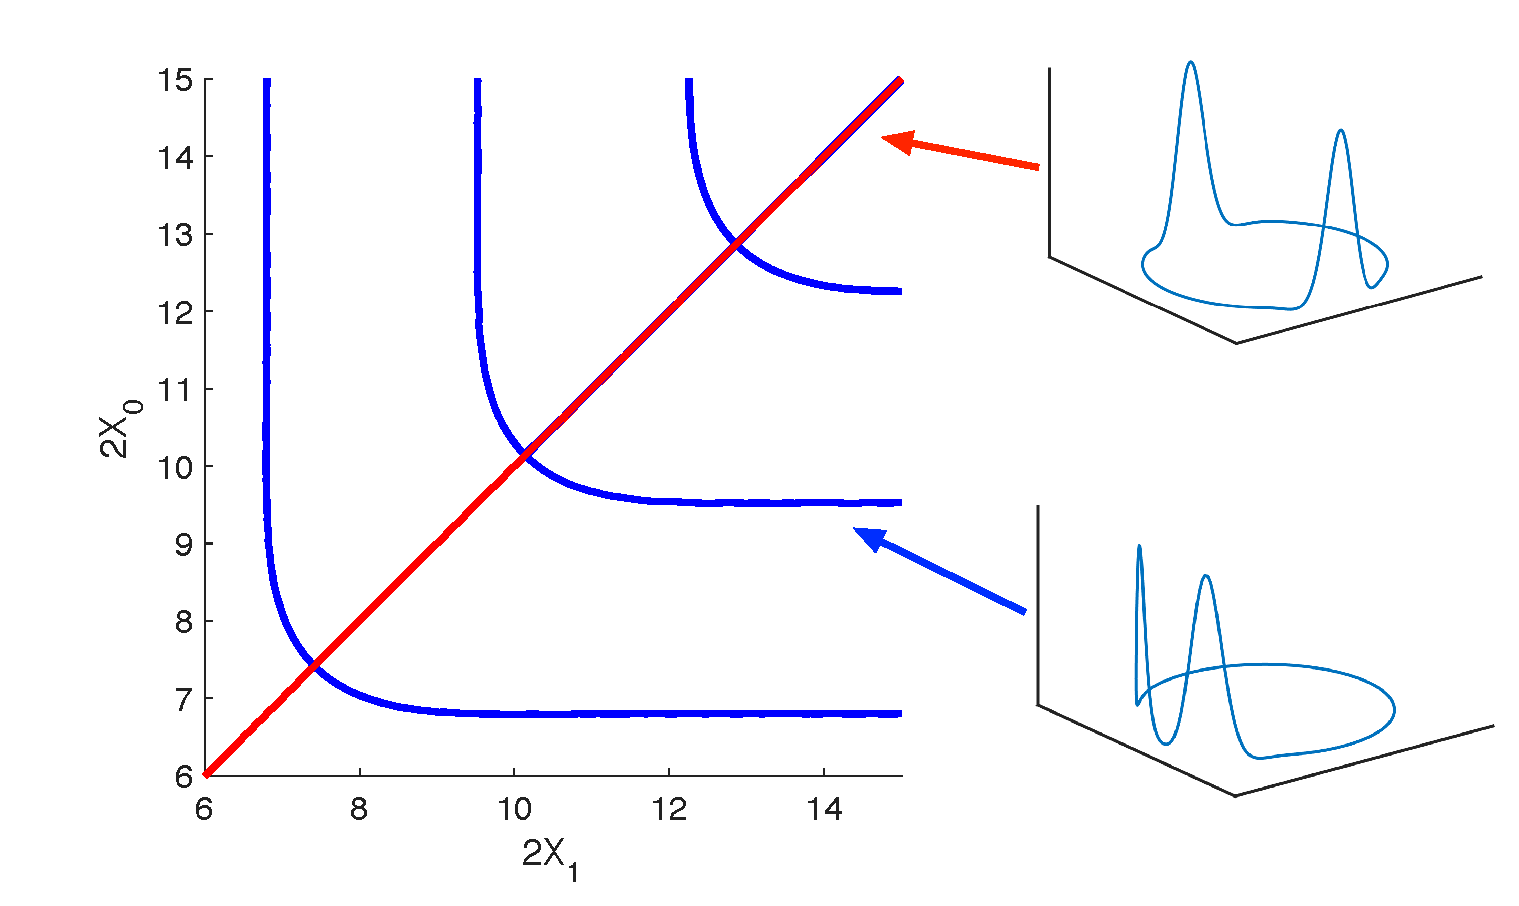
\includegraphics[width=10cm]{periodicpitchforklabeled.eps}
\caption{Asymmetric periodic 2-solitons (blue) bifurcate from symmetric periodic 2-solitons (red). The distances between the two solitons are $2X_0$ and $2X_1$.
}
\label{fig:perpitchfork}
\end{center}
\end{figure}

Next, we look at the interaction eigenvalues corresponding to these periodic 2-solitons. To do this, we adapt Lin's method as in \cite{Sandstede1998}. The additional complication in this case is the presence of a one-dimensional center subspace on which solutions may not decay exponentially. For the symmetric 2-solitons, the interaction eigenvalues are a pair of eigenvalues which are either real or purely imaginary. These collide and switch stability in a series of Hamiltonian-Hopf bifurcations which occur at the pitchfork bifurcation points. This is shown in \cref{fig:periodicequaleigbif}.

\begin{figure}[ht]
\includegraphics[width=10cm]{periodicequaleigbif}
\caption{Real (blue line) and imaginary (red line) parts of interaction eigenvalues versus pulse distance ($2 X_1$) for symmetric periodic 2-solitons.}
\label{fig:periodicequaleigbif}
\end{figure}

Finally, we look at the eigenvalues corresponding to asymmetric periodic 2-solitons. I can prove that in most cases, there is a pair of interaction eigenvalues which are either real or purely imaginary. The eigenvalue pattern is shown in \cref{fig:2periodiceigpattern}.

\begin{figure}[ht]
\includegraphics[width=10cm]{2periodiceigpattern.eps}
\caption{Interaction eigenvalue pattern for most periodic 2-pulses. Blue lines represent periodic 2-pulses with a pair of real interaction eigenvalues. Red lines represent periodic 2-pulses with a pair of purely imaginary interaction eigenvalues. Hamiltonian-Hopf bifurcations take place at the black dots.}
\label{fig:2periodiceigpattern}
\end{figure}

There is, however, an important exception to this pattern. Consider an asymmetric periodic 2-soliton with purely imaginary interaction eigenvalues (red pitchfork branches in \cref{fig:2periodiceigpattern}). As the periodic domain size $L$ is increased, the interaction eigenvalue remains (roughly) constant on the imaginary axis, but the purely imaginary eigenvalues corresponding to the essential spectrum move towards the origin. Eventually, there will be a collision between these two eigenvalues. I observe numerically that when this occurs, there is a brief ``instability bubble'' where the two eigenvalues collide, move off of the imaginary axis temporarily, and then recombine. I call these Krein bubbles, since they result from the collision of two imaginary eigenvalues with opposite Krein signature. This is shown in \cref{fig:kreinbubble1}.

\begin{figure}[ht]
\centering
\begin{tabular}{c}
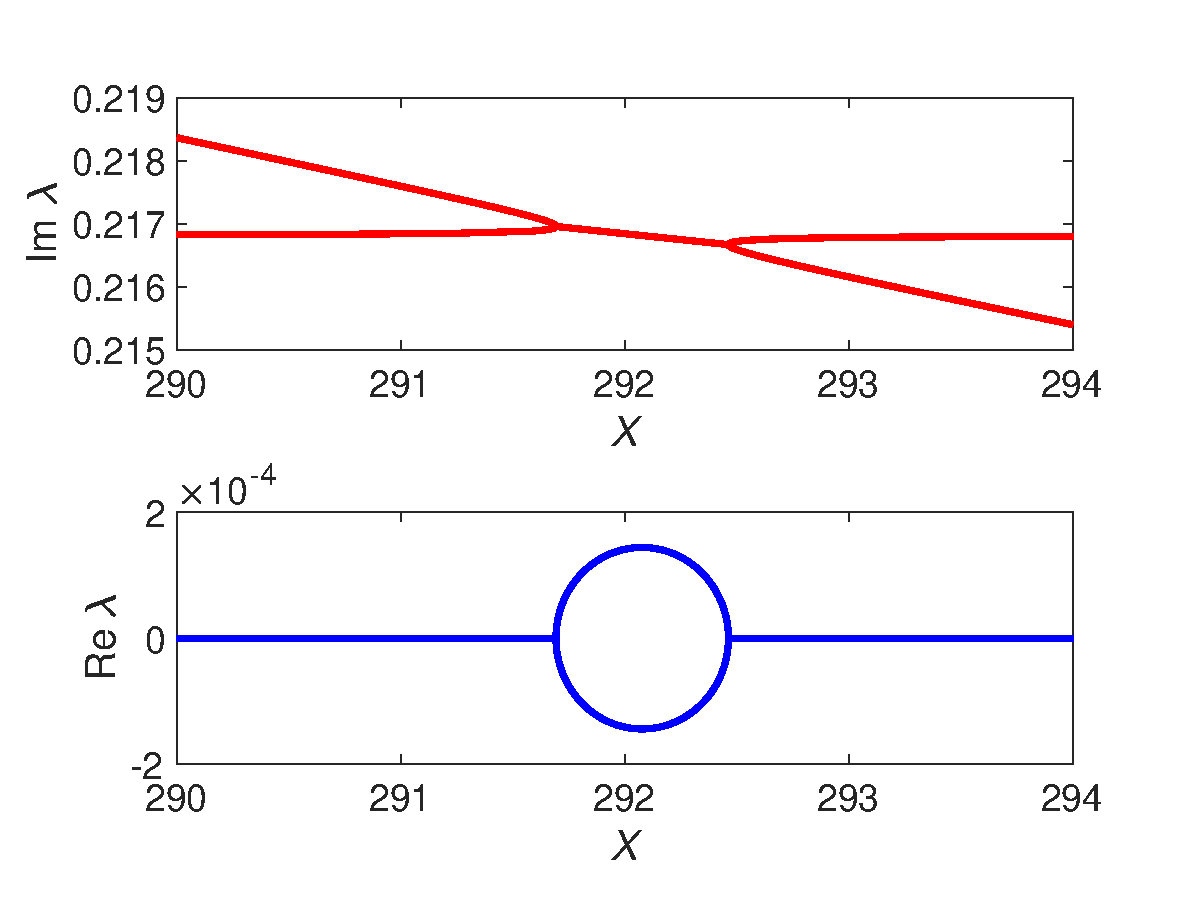
\includegraphics[width=10cm]{kreinbubble1}
\end{tabular}
\caption{Collision of first essential spectrum eigenvalue with purely imaginary interaction eigenvalue as domain size $L$ is increased. Imaginary part of eigenvalues on top, real part of eigenvalues on bottom. Numerical analysis is done with AUTO.}
\label{fig:kreinbubble1}
\end{figure}

Numerical analysis suggests that the Krein bubbles scale with $L^{-1/2}$. I can also prove that if the Krein bubbles occur, they have a maximum radius which is sufficiently small so that the eigenvalue pattern in \cref{fig:2periodiceigpattern} holds in most cases. I am working on proving criteria for these Krein bubbles to exist.

\section{Chen-McKenna suspension bridge equation\footnote{Work with Todd Kapitula and Bj\"{o}rn Sandstede}}

Motivated by observations of traveling waves on suspension bridges, Chen and McKenna \cite{Chen1997} proposed the model
\begin{equation}\label{Chen}
\partial_t^2 u + \partial_x^4 u + \mathrm{e}^{u-1} - 1 = 0.
\end{equation}
to describe waves propagating on an infinitely long suspended beam. There is good evidence that a symmetric, exponentially localized solution $u(x)$ exists for all wavespeeds $c \in (0, \sqrt{2})$ \cite{Smets2002,Berg2018}. Under mild assumptions, which can be verified numerically, this primary soliton solution is orbitally stable. 

I start with numerical analysis. First, I construct the primary soliton using the string method \cite{Chamard2011}. I then glue these together at the appropriate intervals and solve for the multi-soliton using Matlab. Examples of these are shown in Figure \ref{fig:chen1}.
\begin{figure}[ht]
\centering
\begin{tabular}{cc}
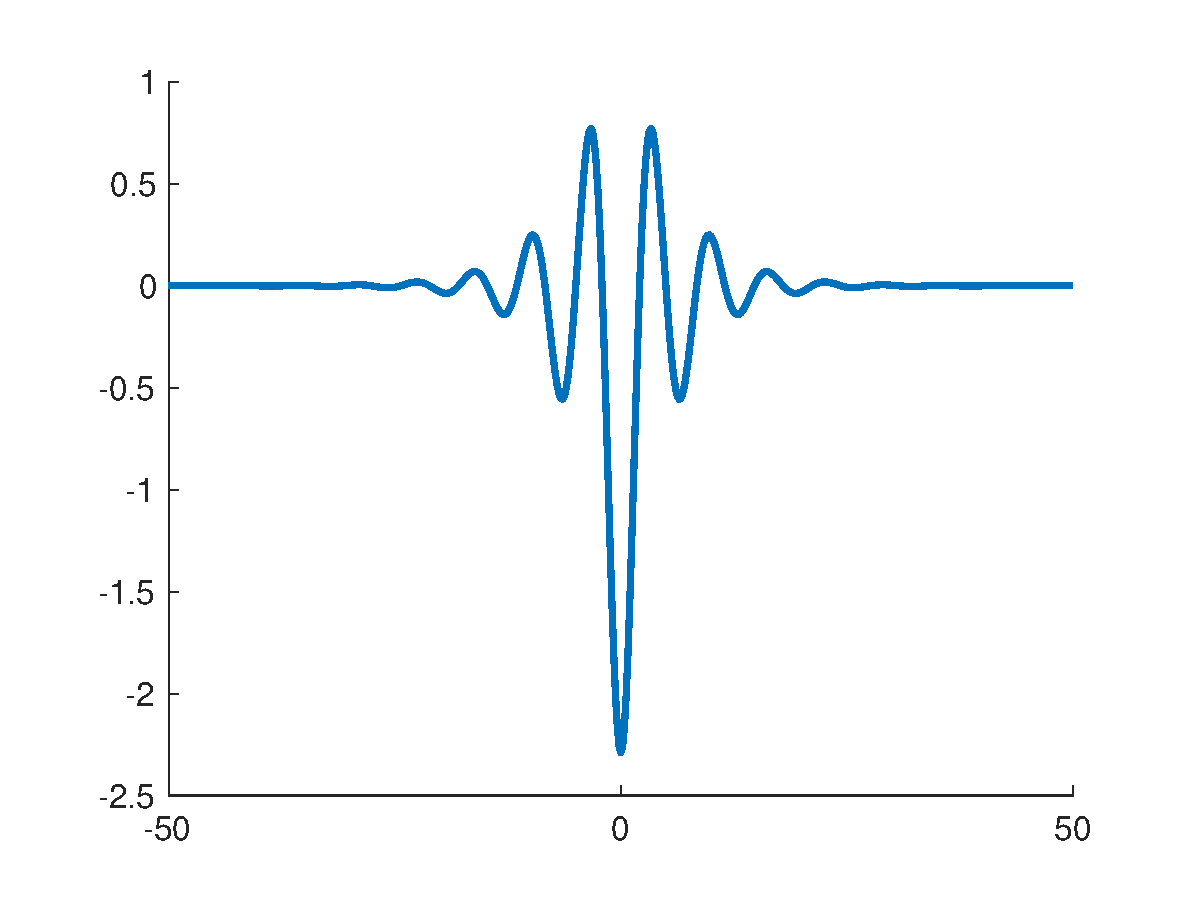
\includegraphics[width=6cm]{single1354}&
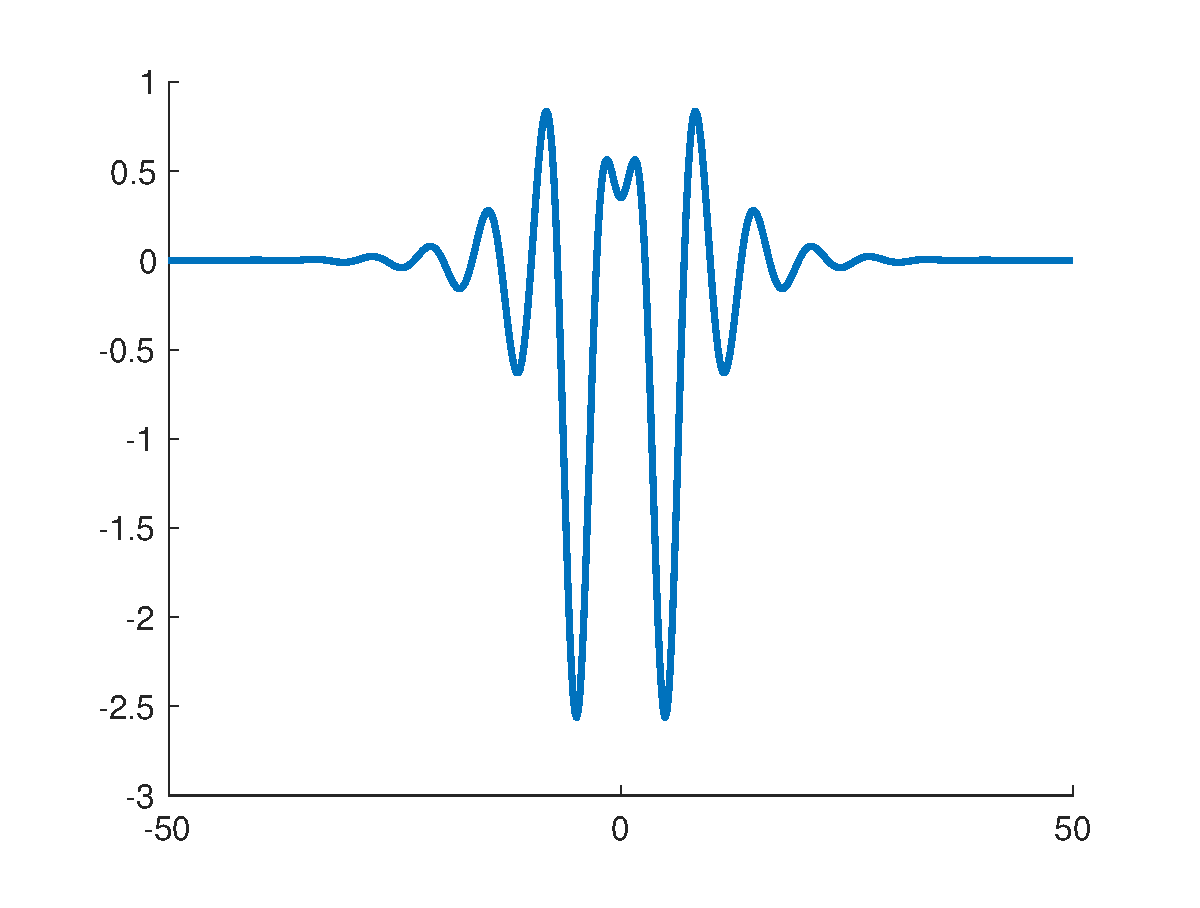
\includegraphics[width=6cm]{double1354}
\end{tabular}
\caption{Primary soliton (left) and double soliton (right) solution to \eqref{Chen}. Finite difference methods, $c = 1.354$.} 
\label{fig:chen1}
\end{figure}
I then use Matlab's eigenvalue solver to find the interaction eigenvalues.

It follows from \cite[Theorem~3.6]{SandstedeStrut} that for each $m \geq 2$, a discrete family of $m-$soliton solutions exists; these solutions can be characterized by a set of $m-1$ nonnegative integers $\{ k_1, \dots, k_{m-1} \}$ in the same manner as multi-soliton solutions to KdV5. 

To determine spectral stability, we linearize the PDE \eqref{Chen} about a multi-soliton solution $u_m(x)$ to get the quadratic eigenvalue problem
\[
[\mathcal{I} \lambda^2 -2 c \partial_x \lambda + (\partial_x^4 + c^2 \partial_x^2 + \mathrm{e}^{u_m(x)})]v(x) = 0.
\]
The essential spectrum is purely imaginary and bounded away from 0, thus spectral stability depends entirely on the point spectrum. To find the point spectrum, we use the Krein matrix to locate the interaction eigenvalues.

The Krein matrix is a Hermitian matrix $\vK(\lambda)$ which is associated with an eigenvalue problem. It is meromorphic in $\lambda$ and has the property that $\det\vK(\lambda)=0$ only if $\lambda$ is a eigenvalue. It can also be used to determine the Krein signature of a purely imaginary eigenvalue. It was introduced in \cite{Kapitula2013a}, and reformulated in \cite{Kap2019} so that it applies to a broader class of problems which include quadratic eigenvalue problems. For the linearization about an $m$-soliton, I showed that the Krein matrix is an $m \times m$ diagonally dominant matrix. The interaction eigenvalue can then be determined from the diagonal entries of the Krein matrix. We then use an eigenvalue counting argument (the Hamiltonian-Krein index) to show that there are no other potentially unstable eigenvalues. The following theorem summarizes the main result.

\begin{theorem}\label{Cheneigs}
Let $u_m(x)$ be an $m$-pulse equilibrium solution to \eqref{Chen} constructed using the sequence of nonnegative integers $\{ k_1, \dots, k_{m-1} \}$. Then
\begin{itemize}
\item For each $k_j$ odd there is a pair of purely imaginary eigenvalues with negative Krein signature.
\item For each $k_j$ even there is a pair of real eigenvalues.
\item There is a geometrically simple eigenvalue at $\lambda = 0$.
\item All other point spectrum is purely imaginary with positive Krein signature.
\end{itemize}
\end{theorem}

\section{Discrete nonlinear Schrodinger equation\footnote{Work with Panos Kevrekidis and Bj\"{o}rn Sandstede}}

The discrete nonlinear Schrodinger equation (dNLS) is the discrete analogue to the nonlinear Schrodinger equation (NLS) and has applications to nonlinear optics and condensed matter physics. In a co-rotating frame, the dNLS equation is
\begin{equation}\label{dNLS}
i\dot{u}_n + d(u_{n+1} - 2 u_n + u_{n-1}) - \omega u_n + |u_n|^2 u_n = 0,
\end{equation}
where $d$ is a coupling parameter; $d > 0$ is the focusing case, $d < 0$ is the defocusing case, and $d = 0$ is the anti-continuum limit (no coupling). 

I am interested in soliton solutions, which are localized equilibrium solutions. For $d > 0$, dNLS has two real-valued, symmetric, soliton solutions (up to translation on the lattice and rotation): an on-site soliton $q_n$, which is centered on a single lattice point; and an off-site soliton $\tilde{q}_n$, which is centered between two adjacent lattice points \cite{Kevrekidis2009}. Since only the on-site soliton $q_n$ is stable, I am interested in the stability of multi-solitons constructed from the on-site soliton solution.

Near the anti-continuum limit, the existence and spectral stability of multi-soliton solutions is known \cite{Pelinovsky2005}. In my work, I prove that these same results hold away from the anti-continuum limit, as along as the individual pulses are well-separated. To do that, I use Lin's method to construct both the multi-solitons and the eigenfuctions associated with the interaction eigenvalues. Since dNLS is invariant under rotation, $e^{i \theta} q_n$ is also a soliton solution. To construct an $m$-soliton, I glue together the $m$ solitons $\{ e^{i \theta_1} q_n, \dots, e^{i \theta_m} q_n \}$ sufficiently far apart. The $m$-soliton is characterized by the pulse distances $\{N_1, \dots, N_{m-1} \}$, which is how many lattice points are between consecutive peaks, and the phase differences $\{ \Delta \theta_1, \dots, \Delta \theta_{m-1}\}$, where $\Delta\theta_j = \theta_{j+1} - \theta_j$. The following theorem summarizes the main results.

\begin{theorem}\label{dNLSeigtheorem}
There exists a positive integer $N$ such that
\begin{enumerate}
\item For any pulse distances $N_j \geq N$ and any phase differences $\Delta_j \in \{0, \pi\}$, there exists a corresponding $m$-soliton equilibrium solution $q_n^m$ to dNLS. No other phase differences are possible.
\item Assume that $M > 0$, where $M$ is the Melnikov sum
\[
M = \partial_\omega \left( \frac{1}{2} \sum_{n=-\infty}^\infty q_n^2 \right).
\]
Then the linearization of \eqref{dNLS} about $q_n^m$ has $m-1$ pairs of interaction eigenvalues $\{\pm \lambda_1, \dots, \pm \lambda_{m-1}\}$ which can be grouped as follows:
\begin{itemize}
\item For each $j$ with $\Delta\theta_j = 0$, there is a pair of real interaction eigenvalues.
\item For each $j$ with $\Delta\theta_j = \pi$, there is a pair of purely imaginary interaction eigenvalues.
\end{itemize} 
\end{enumerate}
\end{theorem}

Lin's method also gives a formula to compute the eigenvalues to leading order. For an $m$-pulse, this involves finding the eigenvalues of an $m\times m$ matrix whose entries only depend on the values of the primary pulse solution $q_n$. In certain special cases, we can obtain a concise formula for the interaction eigenvalues which has good accuracy for intermediate values of the coupling parameter. This is shown in \cref{fig:dNLS3pulseerrors}, where for $d$ between 0.25 and 1, the relative error is less than $0.001$.

\begin{figure}[ht]
\centering
\includegraphics[width=6cm]{dNLS3pulseerrors}
\caption{Log of relative error between leading order computation of interaction eigenvalues via Lin's method and computation of eigenvalues using Matlab's eigenvalue solver. Eigenvalues of a 3-soliton with pulse distances $N = 8$ and phase differences $\Delta \theta = \pi$.} 
\label{fig:dNLS3pulseerrors}
\end{figure}

\bibliographystyle{amsplain}
\bibliography{researchstatement.bib}

\end{document}
